\documentclass{article}

\newenvironment{proof}{\par \noindent {\bf Proof:}}{\begin{flushright}$\Box$\end{flushright}\par \noindent}
\newtheorem{theorem}{\bf Theorem}
\newtheorem{definition}[theorem]{\bf Definition}
\newtheorem{lemma}{\bf Lemma}
\newtheorem{corollary}[theorem]{\bf Corollary}
\newcommand{\pari}{\hspace{\parindent}}

\usepackage{amsmath}
\usepackage{latexsym}
\usepackage{amssymb}
\usepackage{listings}
\usepackage{tikz}
\usepackage{graphicx}
\usepackage{pdfpages}
%\usepackage[pdftex]{graphicx}
%\usepackage{natbib}

\begin{document}

\title{Constrained Optimization Modelling on Resource Allocation for Heterogenous Distributed Systems\footnote{M.Res. Research Project, Department of Computing, Imperial College London} }

\author{Teng Yu\footnote{Corresponding email: {\it t.yu15@imperial.ac.uk}}}
\date{1st Jan. 2016}

\maketitle
\newpage

\begin{abstract}
%{\it The abstract is a very brief summary of the report's contents. It should be about half page long. Somebody unfamiliar with your project should have a good idea of what it is about having read the abstract alone and will know whether it will be of interest to them.}
This work intends to improve the performance of resource allocation process on heterogeneous distributed systems by designing a novel allocation model. It provides a novel approach to involve order theory to model the allocation process and constraints by research on the relations between different resource allocation requests(RAr) and mapping with the structure inside the cluster of servers, then designing ranking functions on their topology as a metric for optimisation instead of viewing the underlining problem as a multi-dimensional bin-packing instance and framing the process as a special Linear Programming formulation which is common in the literature. It focuses on the modelling process and invokes well-known algorithms in experiment to compare its performance with other models. Finally, we discuss that this approach can be easily extended to apply on not only the fields within distributed systems (such as for cloud computing platform), but also in the wide fields of computer science such as for Information Retrieval and HPC.\\\\
%Then we propose to consider a constraint-oriented algorithm, named AC3, to reduce the domain of variables before searching
\end{abstract}
$$ $$
\renewcommand{\abstractname}{Acknowledgements}
\begin{abstract}
%{\it It is usual to thank those individuals who have provided particularly useful assistance, technical or otherwise, during your project. Your supervisor will obviously be pleased to be acknowledged as they will have invested quite a lot of time overseeing your progress.}

First thanks to my parents. Sincere thanks to Dr. Mark Stillwell for his countless helpful comments and advise during this project. Thanks Prof. Alexander L Wolf for his supervision and my personal tutor Dr. Sadri Fariba for advice. Thanks for the Departmental Scholarship funded by the Department of Computing, Imperial College London\\\\
Warm thanks the following friends for their helps and interesting discussions related to this project: Joel Choo (Imperial College London), Shale Xiong (Imperial College London), Jialiang Wang (Harvard University), Bichen Shi (University College Dublin), Huayi Ji (University College Cork), Bojia Ma (City University of Hong Kong) and Hongyu Yang (Eindhoven University of Technology). 
\end{abstract}
$$ $$
\newpage
\tableofcontents
$$ $$
%{\it This should list the main chapters and (sub) sections of your report. Choose self-explanatory chapter and section titles. If possible you should include page numbers indicating where each chapter/section begins. Try to avoid too many levels of subheading. Try if possible to stick to sections and subsections; subsubsections are usually avoidable.}
\newpage
\section{Introduction}
%{\it This is one of the most important components of the report. It should begin with a clear statement of what the project is about so that the nature and scope of the project can be understood by the reader. It should summarise everything you set out to achieve, provide a clear summary of the project's background and relevance to other work, and give pointers to the remaining sections of the report that contain the bulk of the technical material.}

Resource Allocation is a core problem for designing high-performance heterogeneous distributed systems. From a classical point of view, most of approaches in the literature modelled this process as a multi-dimensional bin packing problem\cite{ leinberger1999multi, stillwell2010raa, stillwell2012vmr, rai2012generalized, maguluri2014heavy} whilst powerful heuristics has been developed during the last several decades\cite{panigrahy2011heuristics,caprara2001lower,bansal2006improved}.\\\\
While by considering the nowadays real-world heterogeneous distributed systems, at least one new constraint should be added and one significant constraints has been broken compared with the classical case which also lead to the motivation of the work presented in this report: First, in addition of single resource allocation request (RAr) can contain multiple dimensions such as asking for some CPU capacity and memory space simultaneously, there can also be relations between RArs or say different RArs are not independent; Second, single RAr can ask for the capacity which must be provided by multiple servers simultaneously and then, this also leads to the fact that the difference between RArs may be shown by the relation between servers they needed for. In this case, if we still try to model the scenario as a typical multi-dimensional bin packing problem and solve by linear programming solver, we find the first constraint really increase the complexity of the model as we needed either to adding more dimensions to handle with it\cite{rai2012generalized, ballani2011towards, guo2010secondnet} or update old dimensions and constraints to show the relations\cite{stillwell2012vmr} whilst the second condition thoroughly influence the performance of the solver as not only different balls can be put in one bins, different bins can also be used for one balls.\\\\ 
The novel approach presented in this report share a new light on this problem by focusing on the relations between different RArs and viewing the allocation process as a mapping between the topology of RArs and clusters of servers instead of an action which putting balls into bins. Compared with others pervious approach which also involving set-variables to build up the model\cite{shaw2004constraint}, we consider more theorems from order and lattice theory to construct the efficient model. We first define the relations between the RArs and use partially ordered set ({\it poset}) to represent the initial topology. Then the most interesting achievement we obtained is by originally applying the Birkhoff's representation theory\cite{davey2002introduction} to model this initial topology which precisely transfer the un-modular initial structure to a modular lattice through a bijection. Then, it is easy to design or invoke some ranking functions to label the nodes in this new modular structure and obtains the metrics we needed to analysis the RArs.  We use the MPC-X\cite{mpcx} device by Maxeler Technologies as a concrete industrial example to present our result and show the generality of our theoretical analysis. we have implemented a prototype program based on our model by Java-choco solver\cite{choco3} to compare the performance with the classical bin packing linear-programming model and receive satisfied result, while the main part of model implementation and real data comparison remained to be the future work of this project.\\\\ 
The remaining sections are generated as follow:  section 2 detailed presents the background and related work of resource allocation for distributed systems and show the state-of-the-art. We illustrate the essential knowledge of order and lattice theory used in this work in section 3. The original research is described from the section 4 which gives the definitions of relations between RArs and build up the initial topology of basic independent RArs. Section 5 shows the more general and complicate RArs topology which considering the new conditions. Section 6 analysis our model through the MPC-X device and illustrate the approach by applying Birkhoff's theory, then show the ranking function. The evaluation architecture and results are presented in section 7. We give conclusions and describe the future work in section 8.
   

\section{Background and Related Work}
%{\it The background and related work section of the report should set the project into context by relating it to existing published work that you read at the start of the project when your approach and methods were being considered. There are usually many ways of approaching a given problem, and you should not just pick one at random. Describe and evaluate as many alternative approaches as possible. The published work may be in the form of research papers, articles, text books, technical manuals, or even existing software or hardware of which you have had hands-on experience. Do not be afraid to acknowledge the sources of your inspiration; you are expected to have seen and thought about other people's ideas, so your contribution largely will be putting them into practice in some other context.} 

Modelling on resource allocation problem for variant distributed systems has been widely research in the literature\cite{stillwell2010raa, stillwell2011fdr,stillwell2012vmr, rai2012generalized, guo2010secondnet, ballani2011towards,maguluri2014heavy, vakilinia2015modeling, van2009sla, nguyen2009autonomic,panigrahy2011heuristics,leinberger1999multi}. In this section, we illustrate the work by Stillwell, Vivien and Casanva in 2010 \cite{stillwell2010raa} first as it can be viewed as a common base of the background and related work in a basic homogenous case. Then we extend the discussion to the heterogeneous case by considering servers which can contains different types of resources as illustrated in \cite{stillwell2011fdr} and considering the time-varying and shared-resource need as shown in \cite{rai2012generalized, guo2010secondnet, ballani2011towards}. After that, we presented the practical model designed in \cite{van2009sla,nguyen2009autonomic} and briefly mentioned the recent work in \cite{vakilinia2015modeling} which considered the work-time issue for their model. We discussed the corresponding experimental models in \cite{caprara2001lower, panigrahy2011heuristics} and illustrated the novel modelling approach shown in \cite{shaw2004constraint} which motivated our work in this report. 

\subsection{Model on Homogenous System} 
The work in \cite{stillwell2010raa} detailed illustrated a typical approach to model the problem in a subset of general distributed systems, named the {\it shared hosting platforms}\footnote{Shared hosting platforms can share cluster resources among services to achieve a trade-off between high utilisation and performance isolation\cite{urgaonkar2008agile}}. The authors view the allocation process as a  multi-dimensional bin packing problem, model it as a Mixed Integer Linear Program then invoke different kind of algorithms to solve it and finally, evaluate the performance by some benchmark experiments. The main achievement they obtained is a formulation of this resource allocation problem in such a shared hosting platform for static workloads to make decisions when allocating hardware resources to service instances. As shown in \textbf{Figure \ref{fig:sit}}, they viewed the resource allocation as a bridge between the servers and services to construct the system model. They encapsulated homogeneous servers in cluster with high-speed switched interconnect and each server provided several resources (e.g., CPU, RAM space, I/O bandwidth, disk space) whilst they assumed each service consists of a single Virtual Machine(VM) instance\footnote{The authors also discussed an extension of their result in multi-VM services in section6 of their paper}. 
\begin{figure}
\center
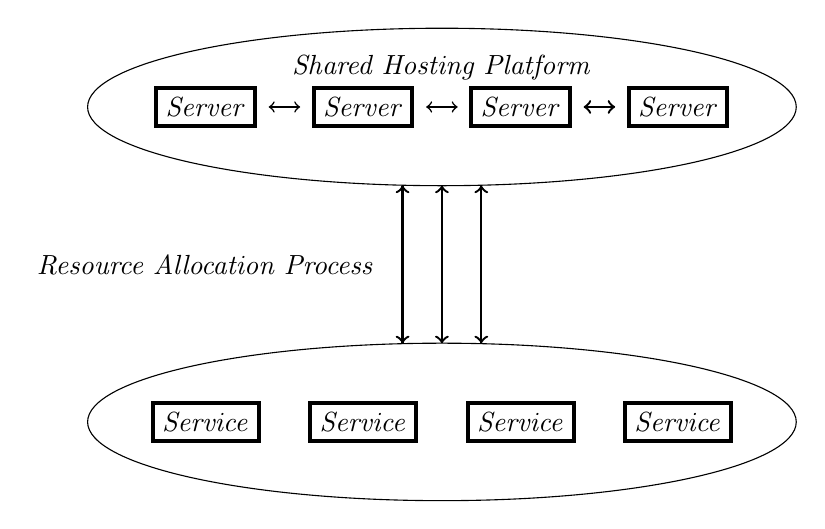
\begin{tikzpicture}
 \node at (3,6.5) {\textit{Shared Hosting Platform}};
\draw (3,2) ellipse (4.5 and 1);
\draw (3,6) ellipse (4.5 and 1);
\node[draw,line width=0.5mm] at (4,6) {\textit{Server}};
\node[draw,line width=0.5mm] at (0,6) {\textit{Server}};
\node[draw,line width=0.5mm] at (2,6) {\textit{Server}};
\node[draw,line width=0.5mm] at (6,6) {\textit{Server}};
\node[draw,line width=0.5mm] at (4,2) {\textit{Service}};
\node[draw,line width=0.5mm] at (0,2) {\textit{Service}};
\node[draw,line width=0.5mm] at (2,2) {\textit{Service}};
\node[draw,line width=0.5mm] at (6,2) {\textit{Service}};
 \draw[<->,line width=0.2mm] (2.8,6) -- (3.2,6);
  \draw[<->,line width=0.2mm] (0.8,6) -- (1.2,6);
   \draw[<->,line width=0.3mm] (4.8,6) -- (5.2,6);
  \draw[->,line width=0.3mm] (3,3) -- (3,5);
  \draw[->,line width=0.3mm] (3,5) -- (3,3);
    \draw[->,line width=0.3mm] (2.5,3) -- (2.5,5);
  \draw[->,line width=0.3mm] (2.5,5) -- (2.5,3);
   \draw[->,line width=0.3mm] (3.5,3) -- (3.5,5);
  \draw[->,line width=0.3mm] (3.5,5) -- (3.5,3);
  \node at (0,4) {\textit{Resource Allocation Process}};
 \end{tikzpicture}
\caption{System Model} 
\label{fig:sit}
\end{figure}
As for resource allocation need, they classified as two types: {\it rigid} and {\it fluid}. A rigid need denote that a specific fraction of a resource is required.  The service cannot benefit from a larger fraction and cannot operate with a smaller fraction.  A fluid need specifies the maximum fraction of a resource that the service can use if alone on the server. The service cannot benefit from a larger fraction, but can operate with a smaller fraction at the cost of reduced performance. For each fluid resource need, they then defined the ratio between the resource fraction allocated and the maximum resource fraction potentially used. They named this ratio the {\it yield} of the fluid resource need. To compare yields across
services with various minimum yield requirements, The {\it scaled yield} of a service is as follows:
\begin{equation*}
\text{scaled yield} = \frac{\text{yield} - \text{minimum yield}}{1 - \text{minimum yield}}\,.
\end{equation*}
After that, they specified the assumptions as summaried below:\\
1) Each service consists of only a single VM instance.\\
2) Each service has constant resource needs.\\
3) The yields of all fluid resource needs are identical.\\
4) Rigid resource need are independent from fluid resource needs\\
5) User concerns, or say higher level metrics are directly related to resource fractions allocated to services\\\\
Followed that, they specified the aim precisely as {\it Maximize the Minimum Yield} under the two constraints below:\\
1) The resource capacities of the servers not be overcome.\\
2) A service inside a single VM instance should be allocated to a single server.\\\\
%After that, we use the same problem specification and the constraints formulation as a Mixed Integer Linear Program (MILP)\footnote{please refer to page 8 in \cite{s1} for those formulation}.
Then, consider the problem formulation as a Mixed Integer Linear Program (MILP). Use $N$ services indexed by $i$, $H$ servers indexed by $h$ which each provides $d$ types of resources. Fractions of these resources can be allocated to services. For each service $i$, $r_{ij}$ denotes its resource need for resource type $j$, as a resource fraction between $0$ and $1$. $\delta_{ij}$ is a binary value that is $1$ if $r_{ij}$ is a rigid need, and $0$ if $r_{ij}$ is a fluid need. Give $\hat{y}_{i}$ to denote the minimum yield requirement of service $i$, a value between $0$ and $1$. Define a binary variable $e_{ih}$ that is $1$ if service $i$ runs on server
$h$ and $0$ otherwise. And define $y_{ih}$ the unscaled yield of service $i$ on server $h$, which must be equal to $0$ if the service does not run on the server.  With these definitions the constraints of our linear program are as follows, with $Y$ denoting the minimum yield:
\begin{eqnarray}
\forall i,h   & \quad e_{ih} \in \{0, 1\}\;, \quad y_{ih} \in \mathbb{Q} \label{eq.c1}\\
\forall i     & \quad \sum_{h} e_{ih} = 1 \label{eq.c3}\\
\forall i,h   & \quad 0 \leq y_{ih} \leq e_{ih} \label{eq.c4}\\
\forall i     & \quad \sum_{h} y_{ih} \geq \hat{y}_{i} \label{eq.c5}\\
\forall h,j   & \sum_{i} r_{ij} (y_{ih} (1 - \delta_{ij})  + e_{ih} \delta_{ij}) \leq 1 \label{eq.c6}\\
\forall i     & \sum_h y_{ih} \geq \hat{y}_{i} + Y (1 - \hat{y}_i)  \label{eq.c7}
\end{eqnarray}
This work also provide a powerful section discussing different types of algorithms they applied to solve the resource allocation problem. They analysis and evaluate the trivial solution by solving the MILP directly, 49 greedy algorithms by combining different service sorting strategies and server picking options, a genetic algorithm based on GAlib library\cite{galib} and 4 vector packing algorithms\footnote{Best Fit, First Fit, Permutation Pack and Choose Pack}. Finally, they proved that the Choose Pack Algorithm with sorting vector lists by decreasing the sum of coordinates was the most efficient approach. We ignore the detailed algorithms analysis\footnote{Please refer to the Appendices section for a brief illustration of the most efficient algorithm, VP\_CPSUM: Vector Packing algorithm using choose packing and sorting ordered by decreasing sum of coordinates} and evaluation part which is far beyond the scope of this report as we focus on the modelling processing of resource allocation.

\subsection{Model on Heterogeneous Systems} 
As a common basic case, the above work was easy to extend for heterogeneous platforms. As discussed in their following work\cite{stillwell2011fdr}, each resource provided in different servers contains two different types of capacities, elementary capacity and aggregate capacity in this heterogeneous platforms. The first capacity represents a single element in one resource dimension whilst the second denotes the total resource capacity counting all elements. For example, a server node comprises 2 cores and single memory will have different elementary and aggregate capacity for CPU but same capacity for memory; A resource allocation request may have different or same need for elementary and aggregate capacity. The aggregate capacity need may also not be an integer multiple of the corresponding elementary capacity need. Compared with the homogenous MILP model in \cite{stillwell2010raa}, it used
different vectors to represent {\it rigid} and {\it fluid} resource allocation need\footnote{The authors renamed those two types of resource allocation needs by {\it requirement} and {\it needs} separately in this paper} instead of involving a binary indicator. It added one more constraint to handle the heterogeneous case by representing the aggregate resource capacities through the sum of resource used from all services on a server node.\\\\
While by considering other part of problems occurred in the heterogeneous systems such as shared-dimensions resource request and dynamic workload, Rai, Bhagwan, and Guha illustrated a novel approach implemented by their resource allocation solver, named {\it Wrasse} in \cite{rai2012generalized}. \\\\
Wrasse solver defined a specification language for resource allocation, which was expressive enough to encode a multitude of allocation problems without using any domain-specific abstractions. In terms of bin-packing with domain agnosticism, they assumed any ball could be assigned to any bin, balls consumed resources provided by bins and did not have different types of balls or bins map to in the problem domain as the basic case. Same as the modelling in \cite{stillwell2010raa, stillwell2011fdr}, Wrasse's abstraction for resource was still a single multi-dimensional resource vector and each bin's resource were mapped to different dimensions in that vector and encoded the constraints using a Boolean variable for each ball-bin combination then only a linear number of variables needed. In addition, by exploiting the language features that one ball could be put in only one bin, it used one integer variable for each ball and this variable was set to a value that represent its bin. \\\\
The novel approach to handle with shared resources was presented by adding new dimensions in the corresponding vectors for those resources to map to. For example, in a scenario in which there are $n$ bins with $k$ resources each, and $m$ shared resources, the Wrasse resource vector has  ($k$ $\ast$ $n$) + $m$ dimensions. Each dimension has a capacity, fixed in the problem specification. They also gave a discussion for considering the conflicting constraints in different dimensions: say a strategy that is optimised for performance may not necessarily meet fault-tolerance requirement. And trivially, if we viewed those conflicts as new shared resources constraints, we could handle them through the above way as well. A special mechanism to solve this problem more efficient was considering {\it friends} and {\it foes} groups: they assigned related balls to the same bin and invoked user-defined function to encourage it by feedback but it cannot direct the search algorithm to explore it. All balls in a friend group would be assigned to the same bin while at least one ball in a foe group would be assigned to a different bin. In addition, total difference could be achieved by using pair-wise foe group. They illustrated network virtualization which extending simple VM placement problem with network bandwidth requirements as a concrete example. They illustrated two pervious example physics frameworks: SecondNet\cite{guo2010secondnet} which used the virtual data centre (VDC). Communicating VMs were placed on servers so that they did not exceed the capacities of network links commenting those servers. Each network link in the data centre was represented as resource dimension with the link capacity as the resource capacity; Oktopus\cite{ballani2011towards} with Virtual Cluster(VC): a virtual star topology with $N$ VMs: a single virtual switch connected all VMs and gave bandwidth requirement associated with each virtual link.\\\\
Then it provided another novel mechanism to model the dynamic workload. Say that assigning a ball to a bin must increase the resource utilization along the appropriate resource dimensions while the static resource utilization cannot model resource utilization that arises from the dynamic assignment of balls to bins. This led to the need of designing a function of the dynamic assignment. One way was also applied user-defined imperative function. There were several practical considerations when designing such a function: Soft constrains: over-constrained scenario may accept solutions where a small fraction of constrains are violated: Give a probability with which the constraint must hold; Pinning: for ongoing process, where new balls are added, old balls evicted over time: Wrasse allows the problem specification to 'pin' some balls to bins so as to not perturb already assigned balls in the system; Number of bins: taking the maximum of the total usage divided by total capacity across all bin-specific resources gives us a lower-bound. High-level operation: for each bin, considers all unallocated balls in parallel. A example of  this case was the Microsoft Assessment and Planning Tool (MAP)\cite{map} which took input VM time-varying requirements as a function of time. For each original resource, it created one resource dimension per time-slot. Updated the scalar resource utilization and time-varying utilization similarly. Server utilization maight exceed temporally capacity by at most 10\%.\\\\
They used real-time pair-wise bandwidth constraint as a concrete example for the case when both shared resources need and dynamic workload had to be considered.They captured the above features to design an utilization function: First stored the traffic matrix and routing information, Wrasse maintained a single variable (per dimension) for the current resource utilization; When a VM was to be placed on a solver, then for every other VM on different server, added the bandwidth requirement between this VM and the other VM on path only up to the lowest common ancestor. For other not been placed, added the requirement between this VM and the other VM on the path from this server to the root of the tree. For every VM that was placed on the same server, subtracted the bandwidth between the VMs for all links from this server to the root.\footnote{For more details of the heuristics they applied in the searching process, please refer to the Appendices section in this report. The interesting approach in this part is beyond the scope of this report.} They also discussed using GPU to make best use of the corresponding hardware: Instead of using CPU, threads computed by GPU can ideally execute the same code-path (on different data), collaborate to increase sharing of the limited on-chip memory and avoid expensive synchronisation and data-dependence.\\\\
Several limitations occurred in Wrasse solver: First Wrasse cannot determine non-existence: Wrasse was sound, but not complete; Second say minimization: Wrasse did not guarantee a 'minimal' solution; Third: Wrasse's modelling was still a non-trivial transformation based on the underlining NP-complete Bin-packing problem.\\\\
While from a more practical point of view, Hien Nguyen Van, Frederic Dang Tran, and Jean-Marc Menaud\cite{van2009sla,nguyen2009autonomic} analysis a more complicate system model, or say architecture, to simulate the resource allocation scenario which is more closed to the really world distributeted infrastructures. Instead of using bins and balls to represent, this model composed by Application Environment (AE), Local Decision Module (LDM), Global Decision Module (GDM) and datacenter which contains physical machines and VMs. Briefly, we can say that AE is faced to the application associated with specific performance goals; An application-specific LDM is associated with each AE to evaluate the process baed on the current workload using service-level metric and generate a utility function of the resource allocation; A GDM is used to interact with each LDM and the real-datacenter. It is the core of this system which contains the Constraint solver to determine the management actions based on the input of LDM's utility functions and datacenter's system-level performance metrics. It works like a black box compared with LDM. We prefer to refer to the fig.2 in \cite{van2009sla} of the system graph.\\\\
There are two utility functions in LDM: a fixed service-level function and a dynamic resource-level function which is communicated with GDM and updated for every iteration. VM allocation vectors in LDM are used for building up the upper bound constraints given by each application.As for the GDM: It involves two sequential process, one for determine VM allocation vectors for each application (VM Provisioning) and then for placing VMs and PMs and achieving optimisation (VM Packing). Beyond the constraints formulations based on the CPU and Memory, an interesting approach in VM Provisioning is using a coefficient to allow the administrator to trade-off between the fulfilment of the performance goals and the cost of operating the required resources. Another interesting method is illustrated during the optimisation process in VM Packing: To minimise the number of migration required to reach the new VM-to-PM assignment, or say minimise the reconfiguration to provide a strategy with few interim steps and maximum degree of parallelism. In conclusion, their work presents an automatic virtual resource management system for practical distributed infrastructures. The main advantages include: it can automate the dynamic provisioning and placement of VMs; support for heterogeneous applications and workloads; support for arbitrary application topology.\\\\
By considering the working-time issue in the resource allocation problem, Shahin Vakilinia, Mustafa Mehmet Ali, and Dongyu Qiu's recent work \cite{vakilinia2015modeling} model the process as a job-scheduling scenario instead. It considers the randomness by involving Poisson processing during service time. Then it solves the new issues aroused by this model which including probability distribution and job blocking. It analysis the different cases for VMs, job sizes and release time, respectively to build their efficient model.

\subsection{Model for Experimental Environment}
The next important part for modelling the resource allocation is designing a efficient experimental model. Alberto Caprara and Paolo Toth's pervious work in \cite{caprara2001lower} used classes of randomly generated instances to model the 2-dimensional case. In detail, they used two variables c,d to represent the bins capacities on different dimensions, respectively. Then used Wj and Vj to represent the weights of item j on different dimensions, respectively. Finally used u.d.[a,b] to represent the uniformly distribution of the value for weights of item in the interval [a,b]. There were eight dimensions in the experimental environment. The dimensions in the first six classes are independently sampled. In classes seven and eight, the dimensions are correlated. They achieve positive correlation by setup the domain of the Vj to be a monotonic function from Wj while achieve negative correlation by setup it to be a inverse function in domain.\\\\
Rina Panigrahy, Kunal Talwar, Lincoln Uyeda, and Udi Wieder in \cite{panigrahy2011heuristics} provided a more powerful approach to extend the pervious model on 2-dimensional case to multi-dimensions by setting any additional pairs of dimensions (2i-1) and (2i) correlated as dimension 1 and 2, while independent with the other dimensions. As for generate negative correlation across all dimensions: Random variables to denote the random distribution of balls in each dimension, totally 2 times of the dimensions. Multiply with an random coefficient from [10,40] and over two. Further noise by adding a random value from [0,1] and ignored the overweight item.\\\\ 
As for defining metrics on the experimental model, Mark Stillwell in \cite{stillwell2010raa} sampled the resource needs from a normal probability distribution and gave the following two metrics: Failure rate (fr) :the percentage of instances for which it fails to find a solution; Distance from bound (dfb): the difference between the achieved minimum yield and lower bound.

\subsection{Model from Set Theory}

Instead of the pervious work we mentioned above, Paul Shaw in \cite{shaw2004constraint} give a new approach by modelling the underlining problem in resource allocation: the bin packing problem from a view of {\it Set Theory}.\\\\
The motivation of this approach is by considering a dedicated constraint and the fact that using pruning and propagation rules with lower bound method to significantly reduce search on traditional one dimensional bin packing problem. The new constraint it obtained is by considering the feature of candidate set of each bin. Trivially, there is a bound that a ball whose size is larger than the bin capacity should not be viewed as in this bin's candidate set. It gives some more precisely mathematical notations to represent the relation and generate this condition to make it dynamically during the searching process. In detail, it gives the formulas of single item elimination and commitment. A important fact it mentioned is that any bin load is equal to the total size to be packed, minus the loads of all other bins as it is the only rule which communicates information between different bins.\\\\ 
Followed that, it illustrated the new model of the problem from the view of {\it Set Theory}: As we know the goal is to assign each variable an element from its domain, then the solution can be viewed as an assignment. During the solution construction, we obtain a partial assignment which is a set of current domains at each step. Then it can views the optimisation process as a domain reduction on variables. And it clearly illustrates that its constraint includes one parameter which is a vector of $n$ element (n is the number of balls) indicating the index of the bin into which it will be placed. It also mentions that it is NP-complete to achieve generalised arc consistency in packing constraint, so instead it describes a not-complete algorithm by considering {\it neighbouring subsets} in candidate sets. It means two sets are neighbouring if there is no other subset  in the candidate set whose items sum to a value strictly between themselves. It implement an linear time (even can be computed in constant time by dynamically updating) algorithm {\it NoSUM} to determine if there is such a interim subset exist. Then it is trivially to prune the problem instance by invoking this algorithm. The new lower bound it involved is by splitting the balls in candidate set into subsets using a constant number and apply the result to partial solutions. In conclusion, this new constraint cut search by orders of magnitude.\\\\
This approach really motivated our work in this report: our basic approach is also by modelling the relation of bins and balls by viewing one as the value in another's domain. In addition to just modelling the underlining abstract bin packing problem from the view of relations between different Sets, we try to model the actual resource allocation process as well and focus on the relations between different resource allocation requests and physical servers topology. Our approach extends the pervious work by applying Order and Lattice Theory instead of just the Set theory as we model more practical constraints including non-independent requests and share-server requests by focusing on the {\it ordering} inside the model's topology.  We first illustrated the essential knowledges used in this project in the following section.





\section{About Order and Lattice Theory}
%{\it The central part of the report typically consists of three of four chapters detailing the technical work undertaken during the project. The structure of these chapters is highly project dependent. Usually they reflect the chronological development of the project, e.g., design, implementation, experimentation, and optimisation, although this is not always the best approach. However you choose to structure this part of the report, you should make it clear how you arrived at your chosen approach in preference to the other alternatives documented in the background. For implementation projects you should describe and justify the design of your system at some high level, for example by using any of the design methods taught during the first- and second-term courses, and should document any interesting problems with, or features of, your implementation. Integration and testing are also important to describe. Your supervisor will advise you on the most suitable structure for these middle sections.}\\\\
In this section, we present the essential underlining theorems used in this work from Order and Lattice Theory. We only indicate the definitions of those theories and statements of the theorems ignoring all the verification to make the report concisely. For detail illustration of the content, we refer to Davey and Priestly's well-known book\cite{davey2002introduction}. 
\subsection{Partial Orders}
\begin{definition}
Let $P$ be a set. An partial order on $P$ is a binary relation $\leq$ on $P$ such that, $\forall$ x, y, z $\in$ $P$,\\
(i) x $\leq$ x,
(ii) x $\leq$ y and y $\leq$ x imply x = y,
(iii) x $\leq$ y and y $\leq$ z imply x $\leq$ z.
\end{definition}

\begin{definition}
A set $P$ equipped with an order relation $\leq$ is said to be an partially ordered set. We use the shorthand poset in this paper.
\end{definition}
The cover-relation between elements of a poset  $P$ is defined as follows: $$\forall x,y \in P. \, x \prec y \Leftrightarrow x \leq y \mbox{ and } \not \exists u. \, x \leq u \leq y.$$ We say that ``$y \mbox{ covers }x$'' or ``$x \mbox{ is covered by }y$''. Also, the notation $x \succeq y$ is used to indicate that $x$ covers $y$, or $x$ is equal to $y$. \\

\begin{definition}
A map $f$ from poset $P$ onto poset $Q$ is called an order-isomorphism iff, $$ \forall x, y \in P, x \leq y\ if\ and\ only\ if\ f(x) \leq f(y)\ in\ Q.$$
Then we say poset P and Q are isomorphic iff there exist an order-isomorphism map between P and Q.
\end{definition}

\begin{definition}
Let $X$ be a set. The power-set $\mathcal{Q}$(X), consisting of all subsets of $X$, is ordered by set inclusion: $$ \forall A, B \in \mathcal{Q}(X),\ A\leq B\ if\ and\ only\ if\ A \subseteq B. $$
\end{definition}

\begin{definition}
Let $P$ be a poset and let $S$ $\subseteq$ $P$. An element x $\in$ $P$ is an upper bound of $S$ if s $\leq$ x for all s $\in$ $S$. A lower bound is defined dually. The least element of the set of all upper bounds of $S$ is called the least upper bound and the greatest lower bound is defined dually as well.
\end{definition}

\begin{definition}
Let $P$ be a poset and let $S$ $\subseteq$ $P$. We say $S$ is a lower set of $P$ iff $\forall$x $\in$ $S$ and y $\leq$ x, then y $\in$ $S$.
\end{definition}

\subsection{Lattices and Valuations}
\begin{definition}
Let $P$ be a poset and let $S$ $\subseteq$ P. An element x $\in$ $P$ is an upper bound of $S$ if s $\leq$ x for all s $\in$ $S$. A lower bound is defined dually. The least element of the set of all upper bounds of $S$ is called the least upper bound and the greatest lower bound is defined dually as well.
\end{definition}
We use x $\sqcup$ y (read x join y) to represent the least upper bound of \{x,y\}, whilst use x $\sqcap$ y (read x meet y) to represent the greatest lower bound of \{x,y\}. We use $\bigvee$S to represent the join of $S$ and $\bigwedge$S to represent the meet of $S$.

\begin{definition}
Let $L$ be a non-empty ordered set.\\\\
If x  $\sqcup$ y and  x $\sqcap$ y exist for all x, y $\in$ $L$, then $L$ is called a Lattice.
\end{definition}

\begin{definition}
Given a lattice $L$. An element $x$ $\in$ $L$ is join-irreducible iff:
$$ x = a \sqcup b\ implies\ x = a\ or\ x = b\ for\ all\ a, b \in L $$ 
\end{definition}

\begin{definition}
A function f on a lattice L, $f : L \rightarrow \mbox{$\cal{R}$}^{+}_{0}$ is a {\it valuation} iff 
$$ \forall x,y \in L. \, f(x \, \sqcap \,  y) + f(x \, \sqcup \,  y) = f(x) + f(y). $$ 
\end{definition}
$$ $$
\begin{definition}
A lattice $L = (P,\sqsubseteq)$ is modular iff $$ \forall x,y,z \in L. \, x \sqsubseteq z \Rightarrow x \, \, \sqcup \,  \,  (y \, \sqcap \,  z) = (x \, \sqcup \,  y) \, \sqcap \,  z. $$
\end{definition}
The following equivalence holds in any modular lattice $L$: \\\\$(i)\ \forall x,y \in L. \, x \succ x \, \sqcap \,  y \Leftrightarrow x \, \sqcup \,  y \succ y. $ \\\\$(ii)\ \forall x, y, z \in L. \, x \succ y \Leftrightarrow x \, \sqcup \,  z \succeq y \, \sqcup \,  z.$


\subsection{Birkhoff's Representation Theory}
\begin{definition}
Any finite modular\footnote{In Birkhoff's original definition, it used {\it distributed lattice} instead and give a corollary saying any distributed lattice is modular. We used the followed result directly in this report as the detail mathematical description of the original theorems and corollary with the corresponding proof is far away beyond the range of this work.} lattice L is isomorphic to the lattice of lower sets of the partial order of the join-irreducible elements of L.
\end{definition}

\section{Basic RArs}
In this section, we discuss the relation between basic resource allocation requests (RArs). We assume RArs are independent between different dimensions in the theoretical case and focus on the relation of RArs in each dimension to build up their foundation model.
\subsection{RArs Relations}
Consider to handle with resource that have difficult-to-represent capacities. User's request may be special on different processing element (heterogeneous)or say the relation between them. Then we find the capacity of a cluster is the set of all allocation request that it can service. Try to give a relation between RArs:
\begin{definition}
Given the relation $\preceq$ between RAr:
$$ \forall \alpha \in a\ cluster\ device, \exists A,B \in RAr, such\ that\ A \preceq B\ \Leftrightarrow \alpha{(B)} \mapsto \alpha{(A)}. $$
\end{definition}
We say $\alpha{(B)}$ is true iff $\alpha$ can service B. Then we can define a parallel relation between RArs as follow:
\begin{definition}
$$ \forall A,B \in RAr, A\npreceq B\ \wedge B\npreceq A\ \Leftrightarrow A \parallel B. $$
\end{definition}
Followed by defining relations between user's requests, we can try to build a closed topology involving those requests. It will be more likely a lattice as we can ordered those requests by inclusion through the relation we just defined. As the topology inside a cluster device can be viewed as a littice as well by considering that the intersection of subset servers in cluster, it leads to a possibility to achieve mappings during the allocating process.\\\\ A trivial approach from the order theory is to consider Birkhoff's representation theory, which says modular lattice can be represented by down-sets of its corresponding partial order composed by join-irreducible elements \cite{davey2002introduction}. Then it is easy to view the RArs as downset of the lattice of cluster topology. Then 
it remains to create a metric or say ranking function to compare the performance between different mapping.
\subsection{RArs Model}
Consider there is a common foundation of all RArs which is  a non resource needed request, we represent it as $\bot$. \\\\ 
Say there are some kind of basic RArs which hold only one dimension of resource need. For instance, one RAr, named $A_{1}$, may only need some CPU capacity for computation while another, named $A_{2}$, just need some memory capacity to record information. It is easy to verify that not all cluster devices which can service $A_{1}$ can service $A_{2}$ and vise versa. So in this case, $A_{1}$ and $A_{2}$ are parallel while $\bot$ $\preceq$ $A_{1}$,$A_{2}$. Then it is also easy to extend this instance to the real case that there will be a large number $n$ of different dimensions of RArs, and we have the following two conditions:
$$1)\ \forall i,j \in n, A_{i} \parallel A_{j} $$ 
$$2)\ \forall i \in n, \bot \preceq A_{i}\ \ \ $$
Now we consider the union of those RArs $A_{i}$. Some more complexed RArs may contain multi-dimensional resource allocation requests, which can be viewed as request different one-dimensional RArs simultaneously and this can be achieve by the union of $A_{i}$. In this way, we can define a n-dimensional RAr as follows:
\begin{definition}
Given $A^{n}$ denote a n-dimensional RAr, then:
$$ A^{n} = (\forall A_{i}\ i\in n) \bigwedge A_{i}. $$
\end{definition}
Finally, we say any kind of resource allocation request can be viewed as a n-dimensional RAr and the topology of RArs model can be built up as a partially order set through the relations we just defined. We give an instance of two-dimensional RAr topology in \textbf{Figure \ref{fig:rar}}. We use $A_{1}(1)$ to represent a one-dimensional RAr which only require 1GHz CPU and $A_{2}(1)$ to represent another one-dimensional RAr requiring 1GB memory. Then $A^{2}(1,1)$ is the union of them and represent a two-dimensional RAr. For easy illustration, we suppose 1GHz CPU and 1GB memory are two atom (or say entry) requests in this instance. As there may be 1.5GHz CPU request in a RAr, we use dash line to denote the relation which contains intern nodes and full line to denote the closed relation.\\\\ 
It is not a supervise that we find the result topology is actually a modular lattice: Each pair of nodes in this topology has a least upper bound and a greatest lower bound whilst all nodes satisfy the modular law presented in Definition 11. We ignore the mathematical proof of this result. \\\\
\begin{figure}
\centering
\begin{tikzpicture}
\node (a0) at (10,2) {$A_{2}(2)$};
\node (a1) at (9,1) {$A_{2}(1)$};
\node (a2) at (8,0) {$\bot$};
\node (a3) at (7,1) {$A_{1}(1)$};
\node (a4) at (6,2) {$A_{1}(2)$};
\node (a5) at (8,2) {$A^{2}(1,1)$};
\node (a6) at (7,3) {$A^{2}(2,1)$};
\node (a7) at (9,3) {$A^{2}(1,2)$};
\node (a8) at (8,4) {$A^{2}(2,2)$};
\node (a10) at (11.5,3.5) {$A_{2}(n)$};
\node (a11) at (10.5,4.5) {$A^{2}(1,n)$};
\node (a20) at (4.5,3.5) {$A_{1}(n)$};
\node (a21) at (5.5,4.5) {$A^{2}(n,1)$};
\node (a100) at (8,7) {$A^{2}(n,n)$};
\draw[dash pattern=on2pt off3pt] (a5) -- (a6);
\draw[dash pattern=on2pt off3pt] (a6) -- (a8);
\draw[dash pattern=on2pt off3pt] (a7) -- (a8);
\draw (a2) -- (a3);
\draw (a2) -- (a1);
\draw[dash pattern=on2pt off3pt] (a4) -- (a3);
\draw[dash pattern=on2pt off3pt] (9,5) -- (a8);
\draw[dash pattern=on2pt off3pt] (7,5) -- (a8);
\draw (a5) -- (a1);
\draw (a5) -- (a3);
\draw (a6) -- (a4);
\draw[dash pattern=on2pt off3pt] (a5) -- (a7);
\draw[dash pattern=on2pt off3pt] (a0) -- (a1);
\draw (a0) -- (a7);
\draw[dash pattern=on2pt off3pt] (a5) -- (a7);
\draw[dash pattern=on2pt off3pt] (a0) -- (a10);
\draw[dash pattern=on2pt off3pt] (a11) -- (a100);
\draw[dash pattern=on2pt off3pt] (a21) -- (a100);
\draw[dash pattern=on2pt off3pt] (a20) -- (a4);
\draw[dash pattern=on2pt off3pt] (a21) -- (a6);
\draw[dash pattern=on2pt off3pt] (a11) -- (a7);
\draw (a10) -- (a11);
\draw (a20) -- (a21);
\end{tikzpicture}
\caption{2-dimensional(CPU, Memory) RAr topology}
\label{fig:rar}
\end{figure}

\noindent{\bf Note:} Instead of the theoretical analysis as above, another way of generating the topology of resource allocation requests, or more generally say {\it informations}, is through real data experiment. One instance of this approach can be refer to \cite{mannila2000global} which tested the web-service requests and also resulted a poset. 

\section{General RArs}
We begin to analysis the general case of RArs topology in this section. In the first subsection, we extend the work in last section by reducing the constraint of independence between different dimensions in a RAr. Then in the next subsection, we consider the scenario where a RAr ask for service from multiple servers simultaneously. 

\subsection{Non-independent RArs Model}
Instead of the two independent dimensions we considered in above section, now let's focus on the case when there are two related dimensions in a single RAr. For instance, we can assume a RAr which need 2{\it Mb/sec} network link's capacity and 3{\it Mb/sec} I/O bandwidth. While it is easy to say any RAr containing network link's capacity need will always need at least the same I/O bandwidth. Then, we say those two dimensions in a RAr are not independent. We use $B_{1}(1)$ to represent a one-dimensional RAr which only require 1{\it Mb/sec} network link's capacity and $B_{2}(1)$ to represent another one-dimensional RAr requiring 1{\it Mb/sec} I/O bandwidth. Then $B^{2}(1,1)$ is the union of them and represent a two-dimensional RAr. Same as the above section, we suppose 1{\it Mb/sec} network link's capacity and 1{\it Mb/sec} I/O bandwidth are two atom requests in this instance. We formalise the relation between those two RAr's dimensions as below:
$$\forall i \in \mathcal{N}^{+}, B_{2}(i) \preceq B_{1}(i)\ \ \ $$
Then it leads to the following corollary:
$$\forall i \in \mathcal{N}^{+}, B_{1}(i) = B^{2}(i,i)\ \ \ $$
Where $\mathcal{N}^{+}$ denotes the set of positive integers. The basic topology of RArs with those two dimensions is shown in \textbf{Figure \ref{fig:rar2}}. Compared with the topology in \textbf{Figure \ref{fig:rar}} with two independent dimensions, this topology is a really general case of a lattice instead of a modular lattice. Say if we use three nodes: $B^{2}(1, 2)$, $B_{1}(2)$ and $B_{2}(3)$ as a triple, then this triple will not satisfy the modular law: $B^{2}(1, 2)$ $\preceq$ $B_{1}(2)$ but $B^{2}(1, 2)$ $\sqcup$ ($B_{2}(3)$ $\sqcap$ $B_{1}(2)$) $\neq$ ($B^{2}(1, 2)$ $\sqcup$ $B_{2}(3)$) $\sqcap$ $B_{1}(2)$. This topology will contains more such non-modular triples or non-modular sub-lattice if adding the values in each dimension.

\begin{figure}
\centering
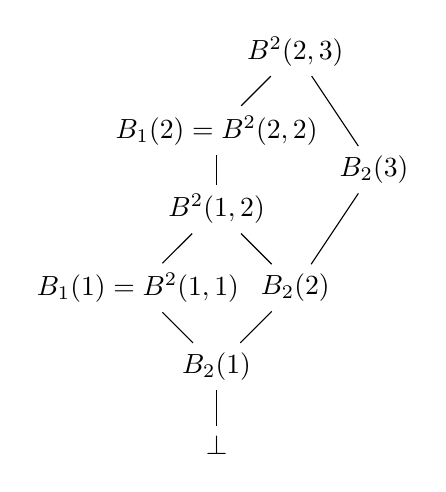
\begin{tikzpicture}
\node (a0) at (2,0) {$\bot$};
\node (a1) at (1,2) {$B_{1}(1)=B^{2}(1,1)$};
\node (a2) at (2,1) {$B_{2}(1)$};
\node (a5) at (3,2) {$B_{2}(2)$};
\node (a4) at (2,3) {$B^{2}(1, 2)$};
\node (a6) at (2,4) {$B_{1}(2)=B^{2}(2,2)$};
\node (a7) at (4,3.5) {$B_{2}(3)$};
\node (a8) at (3,5) {$B^{2}(2, 3)$};
\draw (a8) -- (a7);
\draw (a8) -- (a6);
\draw (a6) -- (a4);
\draw (a5) -- (a7);
\draw (a2) -- (a1);
\draw (a2) -- (a0);
\draw (a1) -- (a4);
\draw (a5) -- (a4);
\draw (a5) -- (a2);
\end{tikzpicture}
\caption{2-dimensional(Network Link, I/O Bandwidth) RAr topology}
\label{fig:rar2}
\end{figure}


\subsection{Multi-server RArs Model}
We consider the case when a RAr can ask for resources provided by different servers simultaneously in this section. From a traditional bin-packing point of view, not only one bin can contains multiple balls but also one ball can be separated and put into different bins in this scenario. Instead of based on some example RArs, we analysis the relation through the general multi-server RArs directly.\\\\
It is interesting to find that when we totally refer to the relations between different multi-server RArs, the topology is much more simple than the above cases as we obtained a trivial linear-order. As shown in \textbf{Figure \ref{fig:rar3}}, we use $S(i)$ to denote a general RAr which ask for $i$ server's resources simultaneously. The linear-order set we obtained is constructed by the trivial relation or say constraint between those RArs, say: $$ \forall i \in \mathcal{N}^{+},\ S(i) \preceq S(i+1) $$
\begin{figure}
\centering
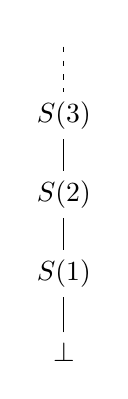
\begin{tikzpicture}
\node (a0) at (2,0) {$\bot$};
\node (a1) at (2,1) {$S(1)$};
\node (a2) at (2,2) {$S(2)$};
\node (a3) at (2,3) {$S(3)$};
\node (a4) at (2,4){};
\draw (a0) -- (a1);
\draw (a2) -- (a1);
\draw (a2) -- (a3);
\draw[dash pattern=on2pt off3pt] (a4) -- (a3);
\end{tikzpicture}
\caption{Multi-server RArs topology}
\label{fig:rar3}
\end{figure}
While the structure becomes complicate when we have to consider the relations between different servers. In the real industrial case, heterogeneous servers will provide different types or amount of resources even the number of them are the same. Further more, the difference between servers more also led by the physics topology they are allocated. For instance, two neighboured servers in a distributed system can provide resources with less network delay and enjoy more traffic tolerance than other pairs of servers. We refer to the next section as a concrete industrial example to illustrate our approach on a real-world distributed system by modelling it as a poset then transferring to a modular lattice. 
\section{MPC-X RArs}
%ask for reference
Now we consider the MPC-X\cite{mpcx} system with the additional constraints between RArs as a practical case. This is a real extended scenario that a RAr can request different server to work for it or say allocate to it simultaneously which break the classical constraints for any bin-packing problem model as they all limit that one ball can only be allocated to exactly one bin.\\\\ In this section, we first briefly describe the topology of MPC-X device and then model the RArs based on its special relations. Finally we discuss some potential approaches to build up metric.
\begin{figure}
\center
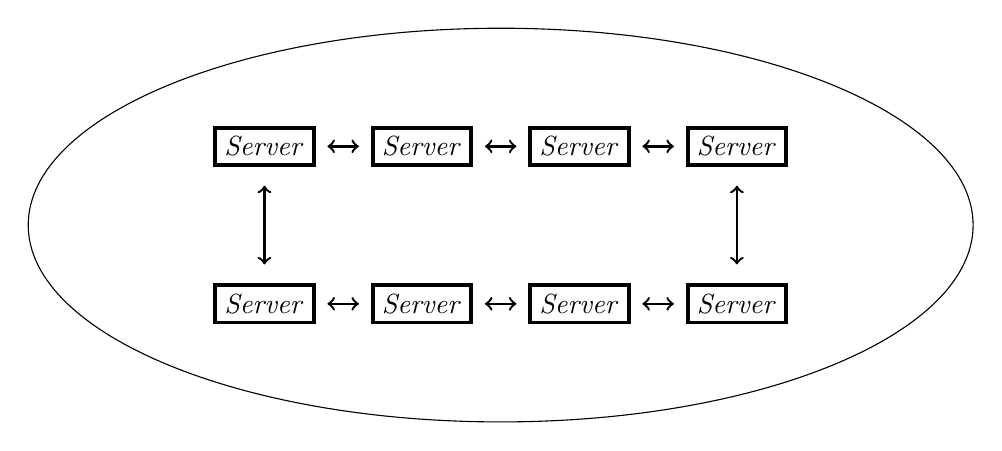
\begin{tikzpicture}
% \node at (3,6.5) {\textit{Shared Hosting Platform}};
%\draw (3,2) ellipse (4.5 and 1);
\draw (3,5) ellipse (6 and 2.5);
\node[draw,line width=0.5mm] at (4,6) {\textit{Server}};
\node[draw,line width=0.5mm] at (0,6) {\textit{Server}};
\node[draw,line width=0.5mm] at (2,6) {\textit{Server}};
\node[draw,line width=0.5mm] at (6,6) {\textit{Server}};
\node[draw,line width=0.5mm] at (4,4) {\textit{Server}};
\node[draw,line width=0.5mm] at (0,4) {\textit{Server}};
\node[draw,line width=0.5mm] at (2,4) {\textit{Server}};
\node[draw,line width=0.5mm] at (6,4) {\textit{Server}};
\draw[<->,line width=0.3mm] (2.8,6) -- (3.2,6);
  \draw[<->,line width=0.3mm] (0.8,6) -- (1.2,6);
   \draw[<->,line width=0.3mm] (4.8,6) -- (5.2,6);
   \draw[<->,line width=0.3mm] (2.8,4) -- (3.2,4);
  \draw[<->,line width=0.3mm] (0.8,4) -- (1.2,4);
   \draw[<->,line width=0.3mm] (4.8,4) -- (5.2,4);
   \draw[<->,line width=0.3mm] (0,4.5) -- (0,5.5);
  \draw[<->,line width=0.3mm] (6,4.5) -- (6,5.5);

\end{tikzpicture}
\caption{MPC-X device}
\label{fig:mpc}
\end{figure}

\subsection{MPC-X topology and RAr relations}
An abstract MPC-X device contains eight servers arranged in a ring as shown in \textbf{Figure \ref{fig:mpc}}. We assume the servers are homogeneous in a device. Then there are two types of RArs: one for singleton servers whilst another for adjacent servers. We use $S_{n}$ (n=1...8) to represent the first type RArs while $A_{n}$ (n=1...8) to represent the second and in both of them, the index represent the number of server it requested.\\\\
Then it is easy to say the foundation relation below:
$$1)\ \forall i \in (1,...,n-1), S_{i} \preceq S_{i+1} $$
$$2)\ \forall i \in (1,...,n-1), A_{i} \preceq A_{i+1} $$
$$3)\ \forall i \in (1,...,n), S_{i} \preceq A_{i}\ \ \ \ \ \ \ \ $$
$$4)\ \ \ \ \ \ \ A_{1}=S_{1}\ \ \ \ \ \ \ \ \ \ \ \ \ \ \ \ \ \ \ \ $$
$$5)\ \ \ \ \ \ \ A_{7}=S_{7}\ \ \ \ \ \ \ \ \ \ \ \ \ \ \ \ \ \ \ \ $$
$$6)\ \ \ \ \ \ \ A_{8}=S_{8}\ \ \ \ \ \ \ \ \ \ \ \ \ \ \ \ \ \ \ \ $$
$$5)\ \ \ \ \ \ \ A_{2}\preceq S_{5}\ \ \ \ \ \ \ \ \ \ \ \ \ \ \ \ \ \ \ \ $$
$$6)\ \ \ \ \ \ \ A_{3}\preceq S_{6}\ \ \ \ \ \ \ \ \ \ \ \ \ \ \ \ \ \ \ \ $$

\subsection{MPC-X RAr model}
We give the RArs model of the MPC-X device below \textbf{Figure \ref{fig:rarX}}, ignored the totally-ordered part for easy illustration. As mentioned in section 4.1, we apply Birkhoff's representation theory to map this partial order set to a downset lattice which can be referred to \textbf{Figure \ref{fig:rarXB}}. We use $B_{i}$ to label the graph instead of using the downset label directly to make it more concisely. To illustrate the correspondence, for example, we know $B_{1}$=$S_{2}$ while $B_{14}$ is the downset of $S_{6} \cup A_{4}$ which contains \{$S_{6},S_{5},S_{4},S_{3},S_{2},A_{4},A_{3},A_{2}$\}.\footnote{To keep the main body of this report concisely, we give the detailed table of the corresponding representations between those two topologies in the Appendices section} \\\\
\noindent{\bf Note:} A general result we can inferred from this instance is that the RAr topology from any practical or say industrial distributed systems can be modelled as a modular-lattice by our representation and Birkhoff's theorem.\\\\
Let's then focus on the new modular-lattice model, actually it contains some really additional {\it interesting} nodes which we just ignored in our first MPC-X RAr topology. For instance, we still use the $B_{14}$ we just mentioned above for illustration. There cannot be any single node in the pervious topology to exactly represent the scenario of the union of $S_{6}$ and $A_{4}$. (If we say $A_{6}$, then we find that its capacity is beyond our needs as a scenario in which six servers can work while five of them are adjacent can serve our need but it doesn't satisfy $A_{6}$.) On the other hand, the total sets of node in this new modular-lattice model can represent all the possible scenarios of RAr for the device based on its downward-close character. 

\subsection{Metric on RAr model}
At this step, we can begin to consider a metric on this lattice-model to represent the distance between different RArs to direct the allocation. A common metric on modular-lattice is a {\it valuation}. Recall the formula of valuation in definition 10. A function, or say labelling method which satisfying the valuation law will efficiently show the distance between different RArs as the sum of two different RArs' label will equal to the sum their least upper bound and greatest lower bound. In another word, valuation on the nodes of RArs' lattice topology keep the consistency of ability that to what level of RArs it can serve as shown in the corresponding downset.\\\\
A easy method to compute a valuation is by a ranking function. We refer to Gratzer's book \cite{gratzer2011lattice} for the proof that the following ranking function satisfy the valuation law as it is beyond the range of this work.
\begin{definition}
Let $L$ be a modular lattice. The ranking $f$ on $L$ is a function  $f: L \rightarrow \mbox{$\cal{R}$}^{+}_{0}$ that:
$\forall$ x,y $\in$ $L$: $$(1)\ f(x)=f(y)+1\ \Leftrightarrow y  \preceq x;$$ $$(2)\  f(x)= 0\ \Leftrightarrow x=\bot.$$ 
\end{definition}
This function is easy to compute on any modular lattice in polynomial time complexity, or say within O(nlogn) in which n is the amount of RArs. Based on a greedy approach, we can first define the ranking of a empty RAr to be zero as it must be a bottom in the topology and label the following nodes through binary search\footnote{This is by the case that in modular lattice, one node will connect with at most two nodes in one direction.} in which we labeled by adding one to each child node from its parent node iterately. 
\begin{figure}
\centering
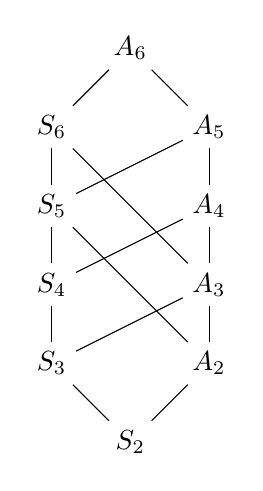
\begin{tikzpicture}
\node (a0) at (2,0){$S_{2}$};
\node (a1) at (1,1) {$S_{3}$};
\node (a2) at (1,2) {$S_{4}$};
\node (a4) at (3,1) {$A_{2}$};
\node (a5) at (3,2) {$A_{3}$};
\node (a6) at (3,3) {$A_{4}$};
\node (a7) at (3,4) {$A_{5}$};
\node (a8) at (2,5) {$A_{6}$};
\node (a10) at (1,3) {$S_{5}$};
\node (a11) at (1,4) {$S_{6}$};
\draw (a0) -- (a1);
\draw (a2) -- (a1);
\draw (a0) -- (a4);
\draw (a5) -- (a4);
\draw (a6) -- (a5);
\draw (a7) -- (a6);
\draw (a7) -- (a8);
\draw (a11) -- (a8);
\draw (a11) -- (a10);
\draw (a2) -- (a10);
\draw (a1) -- (a5);
\draw (a2) -- (a6);
\draw (a7) -- (a10);
\draw (a4) -- (a10);
\draw (a5) -- (a11);
\end{tikzpicture}
\caption{MPC-X RAr topology}
\label{fig:rarX}
\end{figure}

\begin{figure}
\centering
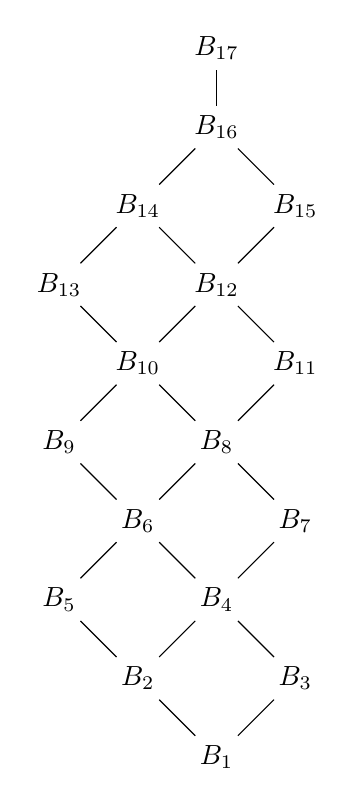
\begin{tikzpicture}
\node (a0) at (2,0){$B_{1}$};
\node (a1) at (1,1) {$B_{2}$};
\node (a2) at (3,1) {$B_{3}$};
\node (a4) at (2,2) {$B_{4}$};
\node (a5) at (0,2) {$B_{5}$};
\node (a6) at (1,3) {$B_{6}$};
\node (a7) at (3,3) {$B_{7}$};
\node (a8) at (2,4) {$B_{8}$};
\node (a10) at (0,4) {$B_{9}$};
\node (a11) at (1,5) {$B_{10}$};
\node (a12) at (3,5){$B_{11}$};
\node (a13) at (2,6) {$B_{12}$};
\node (a14) at (0,6) {$B_{13}$};
\node (a15) at (1,7) {$B_{14}$};
\node (a16) at (3,7) {$B_{15}$};
\node (a17) at (2,8) {$B_{16}$};
\node (a18) at (2,9) {$B_{17}$};
\draw (a0) -- (a1);
\draw (a4) -- (a6);
\draw (a2) -- (a0);
\draw (a1) -- (a4);
\draw (a2) -- (a4);
\draw (a1) -- (a5);
\draw (a4) -- (a7);
\draw (a7) -- (a8);
\draw (a5) -- (a6);
\draw (a6) -- (a8);
\draw (a6) -- (a10);
\draw (a11) -- (a10);
\draw (a11) -- (a8);
\draw (a13) -- (a12);
\draw (a13) -- (a11);
\draw (a8) -- (a12);
\draw (a15) -- (a14);
\draw (a15) -- (a13);
\draw (a17) -- (a15);
\draw (a17) -- (a16);
\draw (a17) -- (a18);
\draw (a14) -- (a11);
\draw (a16) -- (a13);
\end{tikzpicture}
\caption{MPC-X RAr lattice-topology}
\label{fig:rarXB}
\end{figure}


\section{Evaluation}
%{\it All projects need to contain a serious and careful evaluation of their results. The specifics of the evaluation method (e.g., user study, experiments, formal proof review, etc.) are intrinsic to the nature of the project, so this is something that you must discuss and agree with your supervisor early in the project. Ideally, a presentation of the method and results of your evaluation should be included in its own separate section of the report.}\\\\
We illustrate some basic experimental evaluations in this section. Say that we only implement some basic prototype programs at this step of the project. The whole program implementation by the novel model illustrated in this report refer to the future work of this two-term project. 
\subsection{Evaluation architecture}
Two prototype programs are implemented in this step. The first one is a one-dimensional bin packing program by basic linear programming approach. It contains a tiny input size composed by 3 balls and 2 bins. We also implemented a extension vision of this model to handle two-dimensional bin packing problem which is trivially extended from the first one by parallel adding the second dimension. It contains a little larger input size compared with the first one which we used as the basic input instance for multi-dimensional pin packing program. \\\\
Our new model is implemented from the third prototype program which is a one-dimensional bin packing program with the same tiny input size of program one, but the allocation is represented by a lattice which using the domain of bins to represent the balls and the values in the domain to represent the size of each bin.\\\\
We apply the same well-known greedy search algorithm as a benchmark of our following experiment.\\\\ 
All of the programs are implemented in Choco3 solver \cite{choco3} by Java in Eclipse IDE (Vision: Luna Service Release 1a (4.4.1)). The experimental environment is in a MacBook Pro laptop with 2.8GHz Intel Core i7 CPU; 8 GB 1600 MHz DDR3 Memory; and OS X 10.9.2 Operation System. 
\subsection{Evaluation Results}
We first compare the programs through trivial linear-programming bin packing model and our novel model. We show our solutions in the two tables which indicate the statistics results in trivial model and our novel model, respectively. When both of them find the same solution, the model's tuning-time related metrics: building time, Initial propagation and resolution used for program by novel model are all less than the program by trivial model. In addition, the number of constraints applied in our novel model are less than in trivial model.\\\\
The interesting results we find is that our model obtains the efficient solutions although it actually suffers more intern nodes and backtrack and reach larger max depth during the searching process through the same search algorithm. It is corresponding to the fact that the model by lattice when always search all the internal subset during the path even it cannot be the solution.
\begin{table}[t1]
\centering
\begin{tabular}{ |p{0.4cm}||p{1cm}|p{1cm}|p{1cm}|p{1cm}|p{1cm}|p{1cm}|p{1cm}|  }
 \hline
 \multicolumn{8}{|c|}{Statistics Results by Novel Model} \\
 \hline
 No. & Build- ing time & Initial propagation & Reso- lution & Nodes & Back- tracks & Max depth & Cons- traints\\
 \hline
1   & 0.0053s    &0.010s&  0.016s&22&20&21&4\\
2& 0.0052s    &0.009s&  0.016s&22&20&21&4\\
3 & 0.0051s    &0.010s&  0.017s&22&20&21&4\\
4   & 0.0047s    &0.010s&  0.017s&22&20&21&4\\
5& 0.0065s    &0.010s&  0.018s&22&20&21&4\\
6& 0.0054s    &0.009s&  0.016s&22&20&21&4\\
\hline
\end{tabular}
\end{table}

\begin{table}[t2]
\centering
\begin{tabular}{ |p{0.4cm}||p{1cm}|p{1cm}|p{1cm}|p{1cm}|p{1cm}|p{1cm}|p{1cm}|  }
 \hline
 \multicolumn{8}{|c|}{Statistics Results by Trivial Model} \\
 \hline
 No. & Build- ing time & Initial propagation & Reso- lution & Nodes & Back- tracks & Max depth & Cons- traints\\
 \hline
1   & 0.0076s    &0.013s&  0.020s&4&2&3&5\\
2& 0.0076s    &0.014s&  0.019s&4&2&3&5\\
3 & 0.0083s    &0.010s&  0.015s&4&2&3&5\\
4   & 0.0077s    &0.012s&  0.017s&4&2&3&5\\
5& 0.0077s    &0.011s&  0.016s&4&2&3&5\\
6& 0.0078s    &0.011s&  0.016s&4&2&3&5\\
\hline
\end{tabular}
\end{table}


\section{Conclusions and Future work}
%{\it All good projects conclude with an objective evaluation of the project's successes and failures, and suggestions for future work that can take the project further. It is important to understand that there is no such thing as a perfect project. Even the very best pieces of work have their limitations and you are expected to provide a proper critical appraisal of what you have done. Your assessors are bound to spot the limitations of your work and you are expected to be able to do the same.}
This project provides a novel approach to model the resource allocation problem on heterogenous distributed systems by focusing on the relations between resource allocation requests (RArs) and servers. Modelling the resource allocation process as bin-packing problem has been common used in the literature and even viewing this underlining problem from the set theory point of view has been discussed in the pervious work. The novel feature of our work is originally applying Birkhoff's representation theorem from order and lattice theory to represent the topology of RAr as a modular structure which is much more efficient compared with just modelling them as sets and building up constraints through the values in domain. Instead of using linear-programming approach to solve the constrained optimisation problem, our model is constructed based on representation, or say mapping between the structures of RArs and cluster of servers. In this report, we have detailed illustrates the RAr models from the basic homogenous case to the general heterogeneous and practical case. We invoke ranking function on the lattice structure to give metric on the topology and compute the difference between RArs to direct the allocation. \\\\
The main achievement of this project is that we successfully model general heterogenous distributed systems, such as the MPC-X device to a modular lattice instead of a general unconstrained structure. Then we can give easy but efficient metric on RArs to such systems. Our novel model shares a new light on handling resource allocation problem and the underlining multi-dimensional bin-packing problem and specially suited for the case when there are multi-servers RArs and constraints between heterogenous servers.\\\\
We have evaluated the efficiency of our approach in the basic case by solving a trivial bin-packing problem while the implementation of a complicate programme to solve a real resource allocation problem through our model and compare the performance with traditional methods remains to be the future work. Other interesting extensions include applying our model on different practical distributed systems and HPC devices. As our model give a new metric on general RArs, it will also be possible to apply it on an Information Retrieval programme by defining efficient information order and distance.\\\\
The main limitation of our model currently is that it doesn't solve the work-time issue: Our model is based on the bin-packing underlining problem instead of a job-scheduling scenario. Recent work such as \cite{vakilinia2015modeling} model the resource allocation as job-scheduling to handle the work-time issue while our model focuses on the static scenario. It is possible to extend our model to solve job-scheduling problem as well but updating the relations and topology between different RArs may thoroughly reduce the efficiency of this model.
\section{Appendices}
%{\it Appendices contain information that is peripheral to the main body of the report. Information typically included are things like program listings, tables, proofs, graphs, or any other material that would break up the theme of the text if it appeared in situ. Large program listings are rarely required, and should be compressed as much as possible, e.g., by printing in multiple columns and by using small font sizes, omitting inessential detail.}
\subsection{VP\_CPSUM algorithms}
We give high level descriptions of VP\_CPSUM algorithm in this subsection as it is the most efficient methods for the basic homogenous model. We first illustrate the VP\_PPSUM.\footnote{VP\_PPSUM: Vector Packing algorithm using permutation packing and sorting ordered by decreasing sum of corrdinates} below as it provides the basic structure for designing VP\_CPSUM algorithm.
\subsubsection*{VP\_PPSUM algorithm}
1.place each of the N vectors in on of d!/ (d-$\omega$)!  Lists, where $\omega$ $\in$�[1,...,d]\\
 $\Rightarrow$ Each list contains the vectors with a common permutation of their largest $\omega$ dimensions.\\
2.Vectors in each list are then sorted according by decreasing sum of the coordinates (SUM).\\
3.Filling bins with vectors, each time attempting to reduce the resource load imbalance in a bin.\\
$\Rightarrow$ When $\omega$=2, first look in list (i,j) for the first vector that can fit in the bin, hope to reduce the resource imbalance.\\
$\Rightarrow$ If not, relaxes the ordering of the components and searches in other lists.\\
$\Rightarrow$ If no vector can fit in the current bin, then a new bin is added and the process is repeated until all vectors are placed in bins.
\subsubsection*{VP\_CPSUM algorithm}
A relaxation of the VP\_PPSUM algorithm in that it does not enforce any ordering between the $\omega$ coordinates of vectors and thus need only d!/$\omega$!(d-$\omega$)! Lists\footnote{Giving $\omega$=2 leads to good empirical result has been shown in \cite{leinberger1999multi}}. 

\subsubsection*{Bin-centric view}
Rina Panigrahy, Kunal Talwar, Lincoln Uyeda, and Udi WiederFrom in \cite{panigrahy2011heuristics} illustrate the same algorithm\footnote{They named their algorithm as FFDAvgSum which means First Fit by Decreasing Average Sum and is the same as VP\_CPSUM in \cite{stillwell2010raa} } from a bin-centric view: Open only one bin at any time, place items into this bin from the largest suitable one. Close the bin when no item can be put in. Then there are two heuristics by involving random choosing. Grasp[k]: pick a random one from the best k instead of the bext one; Bubblesearch: the kth best is chosen with a propobability proportional to $(1-p)^k$, for a suitable p.

\subsubsection*{Algorithm Analysis}
For fixed d and $\omega$, both algorithm have complexity O(nlogn). In addition, as analysis in \cite{panigrahy2011heuristics}, for the case when some demands in a dimension always dominate the demands in the other dimension, VP\_CPSUM is more robust. The dimensions which are not scare can be assigned smaller coefficients and have a smaller impact on the ordering.

\subsection{Heuristics in Wrasse solver}
This subsection illustrated some heuristics used during the searching processing in the Wrasse solver \cite{rai2012generalized}. Those materials are interested for designing efficient resource allocation algorithm but not closed to the modelling process so we keep them in the Appendices.\\\\
Wrasse invokes the user defined {\it dynamic} utilization function with the partial assignment. In briefly: first checks that capacity constraints are met. After that assign friend balls, check for group-consistency, if violated then left them as unallocated. When no more balls can fit, the solver mores on to the next bin. \\\\
As for the generic search algorithm it used: When picking balls and bins, different choices optimize for difference outcomes. To balance utilization across bins, it uses power of two sized bin-groups, exploit real-world spatial coherence in bins while being domain agnostic. Wrasse solver tries several size in parallel instead of requiring the user to specify in this process and searched the space by exploration: each thread-group independently exploring its own partial solutions as deep as possible. There were four reasons for choosing explore rather than exploit in the wrasse solver: 1. Define 'good' partial solution in a domain-agnostic manner is problematic;  2. We can retain early lucky decisions; 3. After several steps, we end up with a larger diversity of assignments; 4. Do not need addition heuristics.\\\\
Analysis by evaluation: For the VM placement problem, Wrasse is able to match the performance of the carefully tuned, production level placement heuristics. For the network virtualization: Both heuristics find the smallest sub-tree in the network that can for a Virtual Cluster. Wrasse's parallel search for allocations provides high-quality solutions within a few seconds.



%\subsection{Proof of Birkhoff's theorem}

\subsection{Table of MPC-X topology representation}
We provide a detail table of the representation from initial RArs topology of MPC-X device to its corresponding modular lattice topology for easy understanding. Elements in the first column are nodes in the modular lattice after Birkhoff's representation. The second column contains the name of the corresponding downset which the first column denoted. The third column represents the corresponding initial RArs to the MPC-X device which the downset in the second column contains or say the node in the first column can server.
\includepdf[pages=-,pagecommand={},width=\textwidth]{tuuu.pdf}

\subsection{User Guide}
%{\it For projects that result in a new piece of software, you should provide a proper user guide providing easily understood instructions on how to install and use it. A particularly useful approach is to treat the user guide as a walk through of a typical session, or set of sessions, that collectively display all the features of your software. Technical details of how the software works is rarely required. Keep it concise and simple. The extensive use of diagrams illustrating the software in action prove particularly helpful. The user guide is sometimes included as a chapter in the main body of the report, but is often better as an appendix to the main report.}


As illustrated in above section, we use Java-Choco \cite{choco3} solver and Eclipse IDE to implement the experimental programme. We provide a concise guideline in this section about how to install and use it. \\\\
The Java 8 can be downloaded from its official website by Oracle through the following URL: $$ {\it https://www.java.com/en/download/} $$
The Eclipse IDE can be downloaded from the URL: $${\it https://eclipse.org/downloads/ }$$
The Choco solver should be added in the project's referenced libraries and the jar file we used is {\it choco-solver-3.3.3-with-dependencies.jar} which can be free downloaded from the URL: $$ http://choco-solver.org/Download?q=releases$$
The source codes of our prototype programs are open and can be downloaded from the project account in Imperial College's Gitlab: $$ https://gitlab.doc.ic.ac.uk/ty215/MResProjectIC.git $$


\bibliographystyle{plain}
\bibliography{biblio}




\end{document}


\begin{thebibliography}{fi99}

\bibitem[Bes06] {b1} C. Bessiere. Constraint Propagation, Chapter 3 of {\it Handbook of Constraint Programming} (eds. Rossi, van Beek and Walsh), Elsevier, 2006.

\bibitem[Bra13] {b2} F. Brandao, J. P. Pedroso. Bin Packing and Related Problems: General Arc-flow Formulation with Graph Compression. {\it Technical Report DCC-2013-08}, Faculdade de Ci�ncias da Universidade do Porto, Portugal. 2013.

\bibitem[Dav02] {d1} B. A. Davey and H. A. Priestley. {\it Introduction to Lattices and Order} Cambridge
University Press, Cambridge, 2002.

\bibitem[Mac85] {mf} A. K. Mackworth and E. C. Freuder. The complexity of some polynomial network consistency
algorithms for constraint satisfaction problems. {\it Artificial Intelligence}, 25:65-74, 1985.

\bibitem[MM00] {bi} Mannila, H; Meek, C. {\it Global Partial Orders from Sequential Data}, Proceedings of sixth ACM SIGKDD international conference on knowledge discovery and data mining, New York, pp161-168, 2000. 

\bibitem[Pan11] {p0} R. Panigrahy, K. Talwar, L. Uyeda, and U. Wieder. Heuristics for Vector Bin Packing {\it Microsoft Research.} 2011

\bibitem[Pro93] {p1} P. Prosser. Hybrid Algorithms for the Constraint Satisfaction Problem, {\it Computational Intelligence}, Volume 9, Issue 3, pp268-299, 1993.

\bibitem[Rai12] {r1} A. Rai, R. Bhagwan, S. Guha. Generalized Resource Allocation for the Cloud {\it Proceedings of the 3rd Symposium on Cloud Computing}. Oct. 2012

\bibitem[Sch04] {semival} M.P. Schellekens, The correspondence between partial metrics and semivaluations, {\it Theoretical Computer Science}, Volume 315, Issue 1, 5 May 2004, 135–149, 2004. 

\bibitem[Sch14] {syrv} M. Schellekens, T. Yu, S. Romaguera, O. Valero, {\it On Semivaluations and Semimodularity} Domains XI International Workshop on domain theory and applications, Paris, France, 2014.

\bibitem[Sti12] {s0} M. Stillwell, F. Vivien, H. Casanova. Virtual Machine Resource Allocation for Service Hosting on Heterogeneous Distributed Platforms {\it IEEE 26th International Parallel and Distributed Processing Symposium}. 2012

\bibitem[Sti10] {s1} M. Stillwell, D. Schanzenbach, F. Vivien, H. Casanova. Resource Allocation Algorithms for Virtualized Service Hosting Platforms. {\it Journal of Parallel and Distributed Computing}. 2010

\bibitem[Sti08] {s2} M. Stillwell, D. Schanzenbach, F. Vivien, H. Casanova. Resource Allocation using Virtual Clusters. Technical Report ICS2008-09-01, Information and Computer Sciences Dept., University of Hawai'i at Manoa, Sept. 2008

\end{thebibliography}



$$ $$
$$ $$
%{\it Keywords: Resource Allocation, Constraint Optimization, Lattices Theory} \\

%\newpage

%\tableofcontents

\section{Problem Statement}
This work intend to extend the results on resource allocation algorithm in \cite{s1}. We try to involve lattices theory to model the constraints more efficient when framing the resource allocation problem for shared hosting platform. %Then we propose to consider a constraint-oriented algorithm, named AC3, to reduce the domain of variables before searching. Finally, we say this approach can be used to extend the work on dynamic workloads.

\subsection{Problem Specification and Formulation}
We recall the problem specification concisely as mentioned in \cite{s1} in this section. We leave the novel-approach description in the next section. The aim of this work is to design an efficient resource allocation system to control how services share the platform. We first provide the background definitions to describe the problem:\\\\
Each server provides several resources (e.g., CPU, RAM space, I/O bandwidth, disk space) and we consider two kinds of resource needs: {\it rigid} and {\it fluid}. A rigid need denotes that a specific fraction of a resource is required.  The service cannot benefit from a larger fraction and cannot operate with a smaller fraction.  A fluid need specifies the maximum fraction of a resource that the service could use if alone on the server. The service cannot benefit from a larger fraction, but can operate with a smaller fraction at the cost of reduced performance. For each fluid resource need we can define the ratio between the resource fraction allocated and the maximum resource fraction potentially used.  We call this ratio the {\it yield} of the fluid resource need. To compare yields across
services with various minimum yield requirements, we define the {\it scaled yield} of a service as follows:
\begin{equation*}
\text{scaled yield} = \frac{\text{yield} - \text{minimum yield}}{1 - \text{minimum yield}}\,.
\end{equation*}
\\\\
After that, we can specify the assumptions and list them below:\\
1) Each service consists of only a single VM instance.\\
2) Each service has constant resource needs.\\
3) The yields of all fluid resource needs are identical.\\
4) Rigid resource need are independent from fluid resource needs\\
5) User concerns, or say higher level metrics are directly related to resource fractions allocated to services\\\\
Then we specify the aim precisely as {\it Maximize the Minimum Yield} under the two constraints below:\\
1) The resource capacities of the servers not be overcome.\\
2) A service inside a single VM instance should be allocated to a single server.\\\\
%After that, we use the same problem specification and the constraints formulation as a Mixed Integer Linear Program (MILP)\footnote{please refer to page 8 in \cite{s1} for those formulation}.
Finally, we recall the problem formulation as a Mixed Integer Linear Program (MILP). Say we have $N$ services indexed by $i$, $H$ servers indexed by $h$ which each provides $d$ types of resources. Fractions of these resources can be allocated to services. For each service $i$, $r_{ij}$ denotes its resource need for resource type $j$, as a resource fraction between $0$ and $1$. $\delta_{ij}$ is a binary value that is $1$ if $r_{ij}$ is a rigid need, and $0$ if $r_{ij}$ is a fluid need. We use $\hat{y}_{i}$ to denote the minimum yield requirement of service $i$, a value between $0$ and $1$. We define a binary variable $e_{ih}$ that is $1$ if service $i$ runs on server
$h$ and $0$ otherwise. We denote by $y_{ih}$ the unscaled yield of service $i$ on server $h$, which must be equal to $0$ if the service does not run on the server.  With these definitions the constraints of our linear program are as follows, with $Y$ denoting the minimum yield:

\begin{eqnarray}
\forall i,h   & \quad e_{ih} \in \{0, 1\}\;, \quad y_{ih} \in \mathbb{Q} \label{eq.c1}\\
\forall i     & \quad \sum_{h} e_{ih} = 1 \label{eq.c3}\\
\forall i,h   & \quad 0 \leq y_{ih} \leq e_{ih} \label{eq.c4}\\
\forall i     & \quad \sum_{h} y_{ih} \geq \hat{y}_{i} \label{eq.c5}\\
\forall h,j   & \sum_{i} r_{ij} (y_{ih} (1 - \delta_{ij})  + e_{ih} \delta_{ij}) \leq 1 \label{eq.c6}\\
\forall i     & \sum_h y_{ih} \geq \hat{y}_{i} + Y (1 - \hat{y}_i)  \label{eq.c7}
\end{eqnarray}


\section{State of the Art}
Resource Allocation Algorithm on shared hosting platforms has been detailed discussed in \cite{s1}. It provided efficient algorithms to handle the resource allocation problem for a static workload of service by modelling as a constraint optimisation problem. A different approach by using arc-flow formulation with graph compression to solve its prototype problem, {\it the bin packing problem}, has been researched and developed recently in \cite{b2}.\\\\
%While, by considering the domain and relation between the constraints, we try to construct lattices to formulate the constraints more efficient (Section 4.1). Then instead of attempting backtracking which had been shown to be unsuccessful in \cite{s2} and having exponential complexity, we propose to involve a polynomial time method, named Arc consistency \cite{b1} to reduce the domains of variables (Section 4.2). We discuss background techniques and provide the knowledge of lattices on Section 2, recall the definitions in \cite{s1} to specify the problem in Section 3, give a general research plan on Section 5 and remark the proposed work on Section 6.  

\subsection{Background Knowledge}
We shortly recall the background knowledge and techniques beyond the resource allocation problem whilst needed for this work. The detail description of the concepts in the section should be refer to \cite{d1,b1,p1}, respectively. 

%\subsection{Set and Lattices Theory}
\begin{definition}
Let $P$ be a set. An partial order on $P$ is a binary relation $\leq$ on $P$ such that, $\forall$ x, y, z $\in$ $P$,\\
(i) x $\leq$ x,
(ii) x $\leq$ y and y $\leq$ x imply x = y,
(iii) x $\leq$ y and y $\leq$ z imply x $\leq$ z.
\end{definition}

\begin{definition}
A set $P$ equipped with an order relation $\leq$ is said to be an partially ordered set. We use the shorthand poset in this paper.
\end{definition}
The cover-relation between elements of a poset  $P$ is defined as follows: $$\forall x,y \in P. \, x \prec y \Leftrightarrow x \leq y \mbox{ and } \not \exists u. \, x \leq u \leq y.$$ We say that ``$y \mbox{ covers }x$'' or ``$x \mbox{ is covered by }y$''. Also, the notation $x \succeq y$ is used to indicate that $x$ covers $y$, or $x$ is equal to $y$. \\

\begin{definition}
Let $X$ be a set. The power-set $\mathcal{Q}$(X), consisting of all subsets of $X$, is ordered by set inclusion: $$ \forall A, B \in \mathcal{Q}(X),\ A\leq B\ if\ and\ only\ if\ A \subseteq B. $$
\end{definition}

\begin{definition}
Let $P$ be a poset and let $S$ $\subseteq$ P. An element x $\in$ $P$ is an upper bound of $S$ if s $\leq$ x for all s $\in$ $S$. A lower bound is defined dually. The least element of the set of all upper bounds of $S$ is called the least upper bound and the greatest lower bound is defined dually as well.
\end{definition}
We use x $\sqcup$ y (read x join y) to represent the least upper bound of \{x,y\}, whilst use x $\sqcap$ y (read x meet y) to represent the greatest lower bound of \{x,y\}. 

\begin{definition}
Let $L$ be a non-empty ordered set. If x  $\sqcup$ y and  x $\sqcap$ y exist for all x, y $\in$ $L$, then $L$ is called a Lattice.\\\\
\end{definition}


%\subsection{Conflict-Directed Backjumping}
%We describe a more efficient "backtrack" technique named Conflict-Directed Backjumping in the subsection. During a searching process through the space, or say move down through a tree, for each variable, we record in a set the variable which caused the conflict for each value we rejected. We pass back the records of all variable conflicts, and add to the conflict set of the variable we are jumping back to. We delete the conflict sets of any variable we are backtracking from or jumping over.
% and Conflict-Directed Backjumping \cite{p1} to reduce the time complexity during the searching process


\section{Key Research Ideas}

%\subsection{Modelling as Lattices}
Instead of defining a 2-D array $e_{ih}$ to indicate the distribution of each service on each server, we only define an array of servers $s_{h}$ and use the values of those variables to indicate the services allocated on it. In another word, the value of the variable for server is a set of numbers. \\\\
The main advantage of this approach is we can represent the original domain of this variable as a lattice [Bottom, Top] composed by inclusion order or more precisely say power-set as mentioned in definition 3. In this case, the Bottom is \{\} means this server not be allocated to any service whilst the Top is \{1,2,...,N\} means this server is allocated to all services. \\\\
Then some constraints can be easily formulated. For instance, we can represent a service only allocated to a single server by: 
$$ \forall h, \sqcap s_{h} = \{ \} $$ Then state the constraint on the yield of service to resource as: $$ \forall i\in s_{h},\ y_{ih}>0 $$ Follow that, we can use the similar formulations as described in MILP in \cite{s1} to achieve the other constraints.

%\subsection{Reducing domain through Arc Consistency}
%We consider the arc consistency through this approach. As mentioned in section 2.2, we can reduce the domain of all variables in the constraint model (using the MILP or the lattice model mentioned above) to optimise the model itself. AC3 algorithm is a typical algorithm which can achieve a polynomial time complexity. We still need a metric, as $dm$ above to implement the algorithm because it will traverse all possible value of the yield one by one to delete the impossible value. This approach is entirely a pre-processing and will not influence the searching algorithm as well. \\\\
It may be not very meaningful(or say useful) under the condition that all the servers are symmetric and can provide all types of resources, but we can still use it to reduce the domains of yields in this case. While on the other hand, it will be very efficient on a special practical scenario which different servers can provide different types and amount of resources. 

%\subsection{For Dynamic Workloads}

\section{Project Work Plan}
We describe the research plan of the above approach in this section.
%\subsection{Modelling as Lattices}
As for modelling the lattices, The first stage is reading the needed materials in detail. There are two parallel work at the next stage. One is to formulate all the constraints needed based on the lattices-model.  We should define a $discrete\ metric$ ($dm$), or say minimum significant bit when formulating the yield as a lattice. For instance,  if we assume $am$ =10\%, the Top in the domain of the yield-lattice will be \{10\%, 20\%,...1\}. Another work in this step may be implementing a prototype programme such as using the lattice-modelling to solve a basic bin packing, or vector packing problem and design a benchmark to compare the performance with a programme implemented by a typical linear-programming model. The results of this testing should be useful to guide the initial modelling process of the real resource allocation problem.\\\\
The next stage will focus on optimize and implement the lattice model. We need to test a suitable $dm$ and implement the constraints by real coding. Many constraint-solver contains a class of set variable, such as the SetVar in Java-Choco. Then, we need another benchmark to compare the performance of this model with the MILP model under the same searching algorithms, say we don't change the searching method in this approach.\\\\
\subsection{Time Schedule}
Oct. - Nov. Reading the needed materials: focus on [Sti10][Sti12], then other references list below.\\
Nov. - Dec. Formulating the new constraint model and first my first report which including the literature review in detail and the description of the new model before the end of this term.\\
Jan. - Feb. Implementing two prototype programme: one to solve basic bin packing by the new model, two to solve the same problem by classical linear model. Compare the performance and analysis the prototype result (technical report).\\
Feb. - Mar. Implementing the programme to solve the vector packing (which is exactly used for resource allocation)by the new model, compare the performance with the programme used in [Sti10], analysis the result (technical report).\\
Mar. - Apr. More test of the programme by large data (on real-distributed platform if possible) and generate the final report.
%\subsection{Reducing domain through Arc Consistency}
%We first need to design a special AC3 algorithm to deal with the resource allocation problem, a more precise pseudo-code based on the algorithm provided in section 2.2. Some possible applications are using it to reduce the domains of the servers/services/yields. As mentioned in above section, we will not apply it to the domain of servers and services if there is a trivial symmetry for the servers.\\\\
%We plan to implement the perudo-code in the next stage and then following the same methods to test and compare the performance as described in the above subsection. 
%\section{Concluding Remarks}
%This proposal contains two novel approaches to extend the work in \cite{s1} on resource allocation problem.\\\\
%If the first approach can work, then we will obtain a total new model to handle the constraint optimisation for resource allocation problem. This modelling method can be extend to solve other problems in distributed system as well in the future. It is easy to say this method will be more efficient for the case when there are a great number of services allocated to only a few but powerful servers or cluster.\\\\
%If the second approach can work,  we can also obtain a more efficient solution even under the same MILP model and the same searching algorithm. This work is suitable for the case when servers provide different type of resource, or say when some resources are useless or limited in some servers. This approach then open a door to extend the work on dynamic workloads, which means instead of re-compute the total resource allocation algorithm each time, we can repeat the AC algorithm to present the changing of resource need. 





%\subsection{Arc Consistency}
%\begin{definition}
%Let $C_{XY}$ be a constraint between two variables X and Y. \\
(i) A pair (v,w) $\in$ $D_{Y}$$\times$$D_{Y}$ is a support for $C_{XY}$, iff (v,w) $\in$ $C_{XY}$\\
(ii) A value v $\in$ $D_{X}$ is arc consistent w.r.t. $C_{XY}$, iff there is a value w $\in$ $D_{Y}$ s.t. (v,w) is a support for $C_{XY}$\\
(iii) $C_{XY}$ is arc consistent iff for every value v $\in$ $D_{X}$, v is arc consistent w.r.t. $C_{XY}$\\
(iv) A Constraint Satisfaction Problem (CSP) = (V,D,C)\footnote{V: the set of variables; D: the domain of each variable; C: the set of constraints} is arc consistent iff for every constraint $C_{ij}$ $\in$ C, $C_{ij}$ and $C_{ji}$ are arc consistent.
\end{definition}
It is easy to say a value which is not arc consistent cannot appear in any solution of a constraint satisfaction problem. Then it is reasonable to consider this consistent before searching and reduce the domains. The trick in this process is when we remove one possible value, other values in other domains may be inconsistent, so we need a efficient method to iterate. \\\\
A common technique for this problem is named $AC3$ and achieved a polynomial-time complexity: $O(ed^{3})$ in which $e$ is the size of the biggest domain and $d$ is the number of constraints \cite{mf}. We provide a pseudo-code for $AC3$ below:\\\\

\begin{lstlisting}[escapechar=@]
@\textbf{AC3}@(V,D,C)
@\textbf{-----------------------------------------------------------------------}@
@\textbf{for}@ each C@$_{XY}$@ in C
    C @$\gets$@ C + {C@$_{XY}$@}  
  Q @$\gets$@ C
@\textbf{while}@ Q @\textbf{$\neq$}@ {}
    C @$\gets$@ dequeue (Q)
    @\textbf{if}@ revise(C@$_{XY}$@) = true
      @\textbf{if}@ D@$_{X}$@ = {}
          @\textbf{return}@ false
       @\textbf{for}@ each C@$_{ZX}$@ in C, Z@\textbf{$\neq$}@Y
          Q @$\gets$@  Q + {C@$_{ZX}$@} 
@\textbf{return}@ true
@\textbf{-----------------------------------------------------------------------}@
\end{lstlisting}

\subsubsection*{From \cite{stillwell2010raa}:} %s1
Industrial Background: using virtual machine (VM) technology which can consolidate hardware resources to enable shared hosting platforms. \\\\Main achievement: A formulation of the resource allocation problem in shared hosting platform for static workloads to make decisions when allocating hardware resources to service instances.\\\\
System model:  Show in \textbf{Figure \ref{fig:sit}}



One thing to discuss about my report: As for generating the section of background work, I find some parts of literature-review I did is not really closed to main research in my report. Say my project is focusing on the modelling part of the resource allocation instead of algorithms design and analysis. My current approach is separating the materials: for example, I put the knowledge of MILP formulation in your paper in the background section while keep the algorithm description in Appendixes and keep the length of my report through this way. Do you think it make sense? 

$$ $$
Resource and Service model: Each server provides several resources (e.g., CPU, RAM space, I/O bandwidth, disk space) and we consider two kinds of resource needs: {\it rigid} and {\it fluid}. A rigid need denotes that a specific fraction of a resource is required.  The service cannot benefit from a larger fraction and cannot operate with a smaller fraction.  A fluid need specifies the maximum fraction of a resource that the service could use if alone on the server. The service cannot benefit from a larger fraction, but can operate with a smaller fraction at the cost of reduced performance. For each fluid resource need we can define the ratio between the resource fraction allocated and the maximum resource fraction potentially used.  We call this ratio the {\it yield} of the fluid resource need. To compare yields across
services with various minimum yield requirements, we define the {\it scaled yield} of a service as follows:
\begin{equation*}
\text{scaled yield} = \frac{\text{yield} - \text{minimum yield}}{1 - \text{minimum yield}}\,.
\end{equation*}

After that, we can specify the assumptions and list them below:\\
1) Each service consists of only a single VM instance.\\
2) Each service has constant resource needs.\\
3) The yields of all fluid resource needs are identical.\\
4) Rigid resource need are independent from fluid resource needs\\
5) User concerns, or say higher level metrics are directly related to resource fractions allocated to services\\\\
Then we specify the aim precisely as {\it Maximize the Minimum Yield} under the two constraints below:\\
1) The resource capacities of the servers not be overcome.\\
2) A service inside a single VM instance should be allocated to a single server.\\\\
%After that, we use the same problem specification and the constraints formulation as a Mixed Integer Linear Program (MILP)\footnote{please refer to page 8 in \cite{s1} for those formulation}.
Finally, we recall the problem formulation as a Mixed Integer Linear Program (MILP). Say we have $N$ services indexed by $i$, $H$ servers indexed by $h$ which each provides $d$ types of resources. Fractions of these resources can be allocated to services. For each service $i$, $r_{ij}$ denotes its resource need for resource type $j$, as a resource fraction between $0$ and $1$. $\delta_{ij}$ is a binary value that is $1$ if $r_{ij}$ is a rigid need, and $0$ if $r_{ij}$ is a fluid need. We use $\hat{y}_{i}$ to denote the minimum yield requirement of service $i$, a value between $0$ and $1$. We define a binary variable $e_{ih}$ that is $1$ if service $i$ runs on server
$h$ and $0$ otherwise. We denote by $y_{ih}$ the unscaled yield of service $i$ on server $h$, which must be equal to $0$ if the service does not run on the server.  With these definitions the constraints of our linear program are as follows, with $Y$ denoting the minimum yield:

\begin{eqnarray}
\forall i,h   & \quad e_{ih} \in \{0, 1\}\;, \quad y_{ih} \in \mathbb{Q} \label{eq.c1}\\
\forall i     & \quad \sum_{h} e_{ih} = 1 \label{eq.c3}\\
\forall i,h   & \quad 0 \leq y_{ih} \leq e_{ih} \label{eq.c4}\\
\forall i     & \quad \sum_{h} y_{ih} \geq \hat{y}_{i} \label{eq.c5}\\
\forall h,j   & \sum_{i} r_{ij} (y_{ih} (1 - \delta_{ij})  + e_{ih} \delta_{ij}) \leq 1 \label{eq.c6}\\
\forall i     & \sum_h y_{ih} \geq \hat{y}_{i} + Y (1 - \hat{y}_i)  \label{eq.c7}
\end{eqnarray}
$$ $$
About Vector Packing Algorithms:
Resource Allocation Problem is related to the multi-dimensional version of bin-packing, or say vector packing: our service may have fluid resource needs. Attempt to place d-dimensional vectors into (at most) H bins.

\subsubsection*{From \cite{stillwell2011fdr}:}%s0
Focus on the theoretical model: In addition of \cite{stillwell2010raa}, as heterogeneous cases, we consider each server's each resource (or say node's dimension) has two different capacity: Elementary capacity: a single element in each dimension;  Aggregate capacity: total resource capacity counting all elements.
\\\\
Compared the MILP model with \cite{stillwell2010raa}: Using different vector to represent requirement and needs separately instead of invloving a binary indicator. Add one more constraint to represent the aggregate resource capacities achieved by sum the resource used from all services on this node.
\\\\
Still consider the allocation under two constraints: Rigid requirement and fluid need; Both of them become ordered vector pair. Still precisely define the problem as maximize the minimum yield over all services.

\subsubsection*{From \cite{rai2012generalized}:}%r1
A novel approach (Wrasse solver) to resource allocation that permits the problem specification to envelope with ease. The key contribution is defining a specification language for Resource Allocation, which is expressive enough to encode a multitude of allocation problems without using any domain-specific abstractions.\\\\ Specification Language Abstraction: In line with our domain agnosticism, we term objects: balls \& bins respectively. Any ball can be assigned to any bin. Assume not have different types of balls or bins map to in the problem domain.\\\\Abstractions- Resource: Balls consume resources provided by bins. Wrasse?s abstraction for resource is a single multi-dimensional resource vector. Each bin?s resource are mapped to different dimensions in that vector.Shared resources are mapped to yet other dimensions in that vector. For n bins with k resources each, and m shared resources, the Wrasse resource vector has {\it kn+m} dimensions. Each dimension has a capacity, fixed in the problem specification. Face the fact that: there may be conflicting constraints: a strategy that is optimised for performance may not necessarily meet fault-tolerance requirement.
\\\\
Mechanisms- Utilization: Assign a ball to a bin must increment the resource utilization along the appropriate resource dimensions. Problem: Static resource utilization cannot model resource utilization that arises from the dynamic assignment of balls to bins. A function of the dynamic assignment. Require user- defined imperative function. Mechanism - Friends and Foes: It is often desirable to assign related balls to the same bin. User- defined function can encourage it by feedback but cannot direct the search algorithm to explore it. All balls in a friend group will be assigned to the same bin. At least one ball in a foe group will be assigned to a different bin. Using pair-wise foe group to achieve total difference.
\\\\
Practical Considerations: Soft Constrains: Over-constrained scenario may accept solutions where a small fraction of constrains are violated: Give a probability with which the constraint must hold. Pinning: For dynamic ongoing process, where new balls are added, old balls evicted, over time: Wrasse allows the problem specification to ?pin? some balls to bins so as to not perturb already assigned balls in the system. Number of bins: Taking the maximum of the Total usage divided by Total capacity across all bin-specific resources gives us a Cower-bound. Wrasse solver high-level operation: For each bin it considers all unallocated balls in parallel. Invokes the user defined utilization function with the partial assignment. Checks that capacity constraints are met. Assign friend ball, check for group, if violated left as unallocated. When no more balls can fit, the solver mores on to the next bin. Exploiting Language Features: A ball can be put in only one bin: One integer variable for each ball. This variable is set to a value that represent its bin. For best performance, encode the constraints using a Boolean variable for each ball-bin combination. Only a linear number of variables needed
For resource constraints, Wrasse maintains a single variable (per dimension), for the current resource utilization. When allocating ,checks the variables corresponding to the dimensions affected. GPU: To make best use of hardware: Threads should identify execute the same code-path (on different data); They should collaborate to increase sharing of the limited on-chip memory; Avoid expensive synchronisation and data-dependence across threads.
\\\\
Experimental Methodology
Using a collection of randomly generated synthetic problem instances for N services and it servers.
Each service first d/2 resource dimensions, rigid needs.
             last d/2 resource dimensions, fluid needs.
Practical: Same type of need for each individual resource are prevalent

\subsubsection*{From \cite{shaw2004constraint}:}
This paper introduces a dedicated constraint using pruning and propagation rules with lower bound method to significantly reduce search on one dimensional bin packing problem.\\\\ 
Instead of the constraints it gives, we are actually more interested in his problem-model. Comparing with other works, it models the problem from a view of {\it set theory}: It mentions the goal is to assign each variable an element from its domain, then the solution can be viewed as an assignment. During the solution construction, we obtain a partial assignment which is a set of current domains at each step. Then it can views the optimisation process as a domain reduction on variables. And it clearly illustrates that its constraint includes one parameter which is a vector of $n$ element (n is the number of balls) indicating the index of the bin into which it will be placed. This is very similar with our approach as modelling the relation of bins and balls by viewing one is the value in another's domain but from another direction.\\\\
The new constraint it obtains is by considering the feature of candidate set of each bin. Trivially, there is a bound that a ball whose size is larger than the bin capacity should not be viewed as in this bin's candidate set. It gives some more precisely mathematical notations to represent the relation and generate this condition to make it dynamically during the searching process. In detail, it gives the formulas of single item elimination and commitment. A important fact it mentions is that any bin load is equal to the total size to be packed, minus the loads of all other bins as it is the only rule which communicates information between different bins.\\\\
It also mentions that it is NP-complete to achieve generalised arc consistency in packing constraint, so instead it describes a not-complete algorithm by considering {\it neighbouring subsets} in candidate sets. It means two sets are neighbouring if there is no other subset  in the candidate set whose items sum to a value strictly between themselves. It implement an linear time (even can be computed in constant time by dynamically updating) algorithm {\it NoSUM} to determine if there is such a interim subset exist. Then it is trivially to prune the problem instance by invoking this algorithm. The new lower bound it involved is by splitting the balls in candidate set into subsets using a constant number and apply the result to partial solutions. In conclusion, this new constraint cut search by orders of magnitude.

